\documentclass{report}
\usepackage[a4paper, total={17cm, 24cm}]{geometry}
\usepackage{amsmath}

\usepackage{hhline}
\usepackage{bm}
\usepackage{pgfplots}
\usepackage{amssymb}
\usepackage{algorithm}
\usepackage{algorithmicx}
\usepackage{algpseudocode}
\usepackage{color, soul}
\usepackage[backend=biber]{biblatex}
\addbibresource{references.bib}
\graphicspath{{imgs/}}


%opening
\title{Domain Adaptation}
\author{Ash}

\def\BState{\State\hskip-\ALG@thistlm}

\newcommand{\TODO}[1]{\sethlcolor{pink}\hl{\\(#1)\\}}
\newcommand{\FEEDBACK}[1]{\sethlcolor{green}\hl{\\ Feedback: \\#1\\}}
\newcommand{\TOCITE}[2][citation needed]{\textsuperscript{\underline{#1}}}
\newcommand\ddfrac[2]{\frac{\displaystyle #1}{\displaystyle #2}}
\newcommand{\quoteit}[1]{\begin{quote}\textit{#1}\end{quote}}

\begin{document}
	
\chapter*{Domain Adaptation}

\quoteit{Domain Adaptation (DA) allows machine learning methods trained on data sampled from one distribution to be applied to data sampled from another.}
\vspace{3cm}


\subsubsection*{One-Step DA}
The source and target domains are directly related, allowing for knowledge transfer in one step.

\subsubsection*{Multi-Step DA}
Build a series of intermediate bridges to connect two seemingly unrelated domains, then perform one-step DA via this bridge.



\setcounter{chapter}{1}
\chapter*{One-Step Domain Adaptation}
One-step domain adaptation can be categorised into three approaches, each of which can be further split into subcategories as shown in table I.
\begin{figure}[!h]
	\centering
	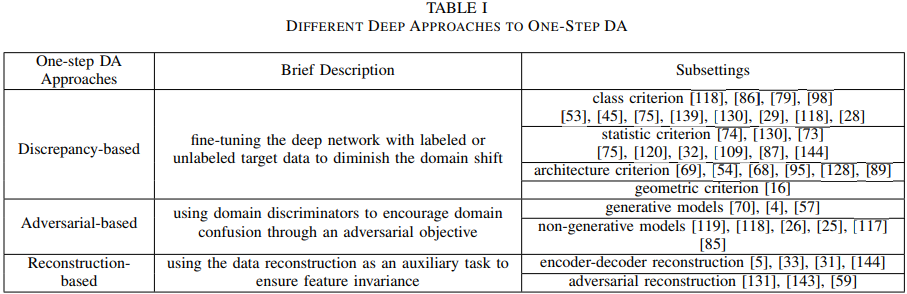
\includegraphics[width=17cm]{one-step-approaches}
	\label{fig:one-step-approaches:1}
\end{figure}


\section{Discrepancy-Based DA}
\quoteit{Assumes that fine-tuning the deep network model with labelled or unlabelled target data can diminish the shift between the two domains.}

\subsection{Class Criterion}
\quoteit{Uses the class label information as a guide for transferring knowledge between different domains. When such samples are unavailable, some other techniques can be adopted to substitute for class labelled data, such as pseudo labels and attribute representation.}

\subsubsection{Soft Label Loss}
Introduced by Geoff Hinton (of course), a ``soft'' softmax can be used when training on the new domain as shown in equation \ref{eqn:softmax:1}, where $T$ is the temperature that's normally set to 1 in standard softmax. Larger values of $T$ produce a softer probability distribution over classes.
\begin{align}
	q_{i} = \ddfrac{exp(z_{j}/T)}{\sum\nolimits_{j} exp(z_{j}/T)} \label{eqn:softmax:1}
\end{align}
Originally used in a paper about distilling knowledge in other networks, using soft labels rather than hard labels can preserve relationships between classes across domains. It is recommended that this is used in conjunction with the domain confusion loss (discussed later). \\ \par

From \parencite{simultaneousdeeptransfer}:
\quoteit{The bottle soft label will have a higher weight on mug than on keyboard, since bottles and mugs are more visually similar. Thus, soft label training with this particular soft label directly enforces the relationship that bottles and mugs should be closer in feature space than bottles and keyboards.}
\quoteit{... we ensure that the parameters for categories without any labelled target data are still updated to output non-zero probabilities.}

\subsubsection{Embedded Metric Learning}
\textit{Unified Deep Supervised Domain Adaptation and Generalization}\parencite{unifieddeepadaptation} uses a siamese network to process source and target domain examples simultaneously, and applies a \textit{Contrastive Semantic Alignment Loss} to the embedded examples, minimising the dissimilarity across domains. \\ \\
\textit{Deep Transfer Metric Learning}\parencite{deeptransfermetric} demonstrates an unsupervised technique for transforming samples into a new subspace. Their training objectives are that:
\begin{enumerate}
	\item the inter-class variations are maximised and the intra-class variations are minimised.
	\item the distribution divergence between the source domain and the target domain at the top layer of the network is minimised.
\end{enumerate}




\subsection{Statistic Criterion}
\quoteit{Aligns the statistical distribution shift between the source and target domains using some mechanisms.}
A frequently used metric is \textbf{Maximum Mean Discrepancy (MMD)}, which estimates the distance between different distributions. 

\subsubsection{Domain Confusion}
\textit{Deep Domain Confusion: Maximizing for Domain Invariance}\parencite{deepdomainconfusion} applies an \textit{adaptation layer} (bottleneck) at some point in the network, then jointly minimises classification error while maximising MMD at the adaptation layer. The minimisation of MMD between source and target domains is known as \textbf{domain confusion}.
\begin{figure}[h]
	\centering
	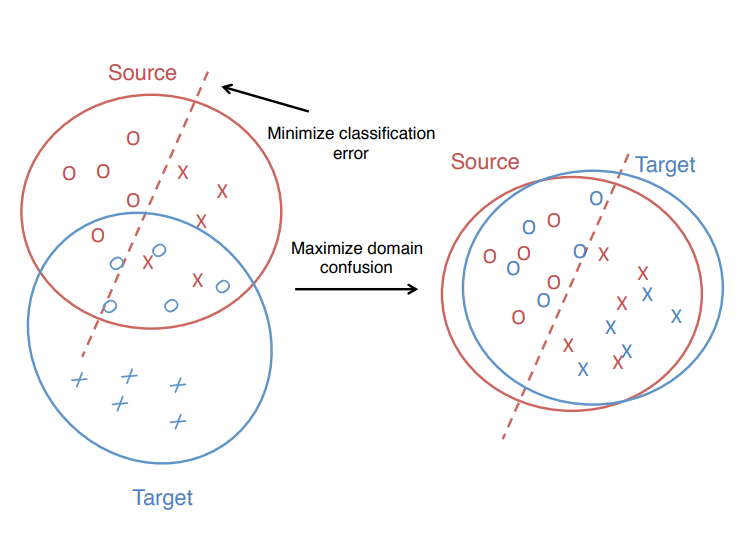
\includegraphics[width=10cm]{domainconfusion}
	\caption{By jointly minimising classification error while maximising domain confusion, we learn representations that are discriminative and domain invariant}
	\label{fig:domainconfusion}
\end{figure}
\begin{figure}[h]
	\centering
	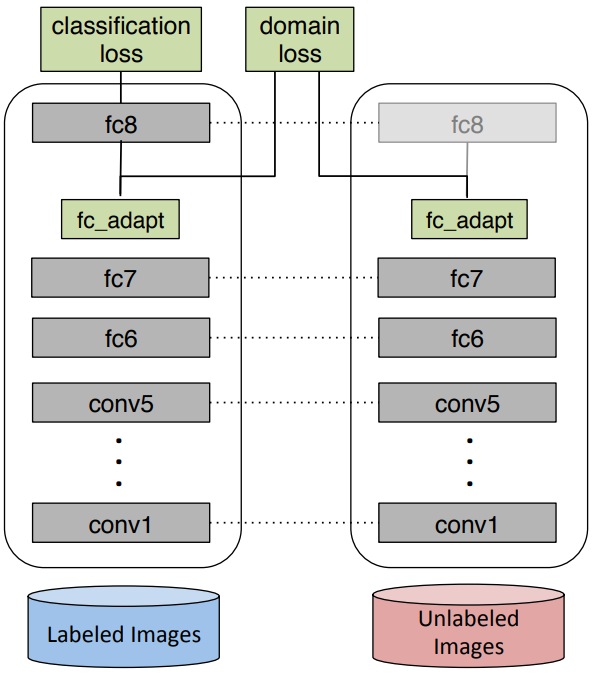
\includegraphics[width=6cm]{imgs/domainconfusion2}
	\caption{Architecture of Deep Domain Confusion\parencite{deepdomainconfusion}}
	\label{fig:domainconfusion2}
\end{figure}
\textit{Learning Transferable Features with Deep Adaptation Networks}\parencite{learningtransferabledeepadaptation} takes it one step further by applying domain confusion to several layers of a network.



\subsection{Architecture Criterion}
\quoteit{Aims at improving the ability of learning more transferable features by adjusting the architectures of deep networks. The techniques that are proven to be cost effective include adaptive batch normalisation (BN), weak-related weight and domain-guided dropout.}

\subsection{Geometric Criterion}
\quoteit{Bridges the source and target domains according to their geometrical properties. This criterion assumes that the relationship of geometric structures can reduce the domain shift.}



\section{Adversarial-Based DA}

\subsection{Generative Models}
\quoteit{The typical case is to use source images, noise vectors or both to generate simulated samples that are similar to the target samples and preserve the annotation information of the source domain}

\subsection{Non-Generative Models}
\quoteit{The feature extractor learns a discriminative representation using the labels in the source domain and maps the target data to the same space through a domain-confusion loss.}



\section{Reconstruction-Based DA}

\quoteit{Assumes that the data reconstruction of the source or target samples can be helpful for improving the performance of DA}

\subsection{Encoder-Decoder Reconstruction}
\quoteit{By using stacked autoencoders (SAEs), encoder-decoder reconstruction methods combine the encoder network for representation learning with a decoder network for data reconstruction}

\subsection{Adversarial Reconstruction}
\quoteit{The reconstruction error is measured as the difference between the reconstructed and original images within each image domain by a cyclic mapping obtained via a GAN discriminator}





\setcounter{chapter}{2}
\chapter*{Multi-Step Domain Adaptation}
Multi-step domain adaptation can be categorised into three approaches as shown in table II.
\begin{figure}[!h]
	\centering
	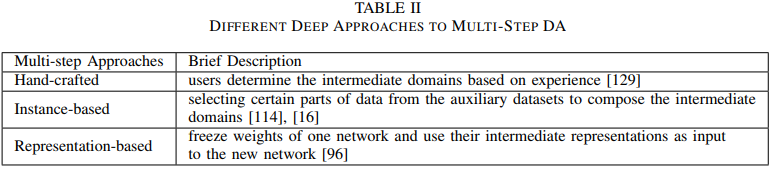
\includegraphics[width=14cm]{two-step-approaches}
	\label{fig:two-step-approaches:1}
\end{figure}
\subsection{Hand-Crafted}
\quoteit{Users determine the intermediate domains based on experience.}
\subsection{Instance-Based}
\quoteit{Selecting certain parts of data from the auxiliary datasets to compose the intermediate domains to train the deep network}
\subsection{Representation-Based}
\quoteit{Transfer is enabled via freezing the previously trained network and using their intermediate representations as input to the new one.}


\chapter*{Application to Swimming Project}

	
\end{document}


